%%%%%%%%%%%%%%%%%%%%%%%%%%%%%%%%%%%%%%%%%%%%%%%%%%%%%%%%%%%%%%%
%
% Welcome to Overleaf --- just edit your LaTeX on the left,
% and we'll compile it for you on the right. If you open the
% 'Share' menu, you can invite other users to edit at the same
% time. See www.overleaf.com/learn for more info. Enjoy!
%
%%%%%%%%%%%%%%%%%%%%%%%%%%%%%%%%%%%%%%%%%%%%%%%%%%%%%%%%%%%%%%%
\documentclass{ctexart}
\usepackage[utf8]{inputenc}
\usepackage{graphicx}
\usepackage{amsmath} % for the equation* environment
\begin{document}
\title{CS61c的讲义简单总结}
\author{lao}
\maketitle
\tableofcontents

\begin{abstract}
大概总结了一下我遇到的cs61c大体知识点
\end{abstract}

\section{整数以及浮点数表示形式}
\subsection{整数的二进制表示方法}
\textbf{这里介绍数字在二进制中的标准存储形式,目的是讲清楚后面在cpu部分中数字的存在形式}\par
首先讲了一会数字可以表示一切的思想,可以跳过然后介绍了一下不同进制之间的转换方法,主要重点在于介绍二进制和十六进制之间转换的优势,提及一个二进制如果位数不是4的倍数我们就往前面填充0达到要求。关于字节:8位一个字节,两个十六进制数,4位一个半子节,一个十六进制数
\begin{figure}
    \centering
    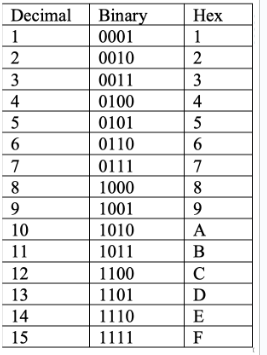
\includegraphics[width=0.5\linewidth]{binary_Hex_convert.png}
    \caption{二进制和十六进制的转换表}
    \label{fig:enter-label}
\end{figure}
\textbf{这里介绍了一下数字向二进制的几种常见转换方法}\par
\textbf{无符号整数转换}最简单的转换方法,方式无需多言,缺点:无法表示负数\par
\textbf{留一个符号位实现兼容负数的改进版}第一位设置为符号位,后面是绝对值缺点:1.一半的地方表示负数去了,正数的范围减半\par2.对正数和负数cpu分别要设计一套处理器,效率很低\par3.存在正0负0\par
\textbf{二进制补码(一种用于表示有符号整数的二进制数系统)}从二进制到数:
第一位乘以-1,其他位正常处理。从数到二进制:对正数正常处理,对负数取负处理然后反转再+1,另外对负数从二进制到数也可以:对负数当正常数处理然后反转再+1
\par 优点:对负数和正数是一套处理器,效率高。\par
\begin{figure}
    \centering
    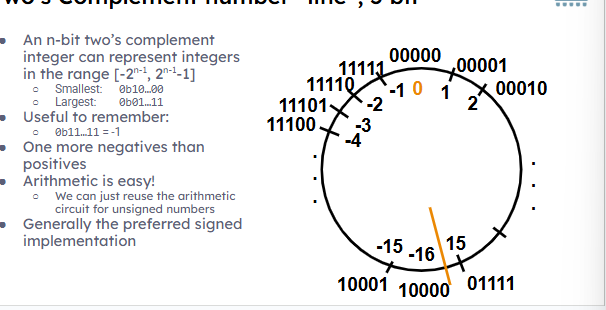
\includegraphics[width=0.5\linewidth]{about two completion you need to know.png}
    \caption{关于二进制补码的常用小知识}
    \label{fig:enter-label}
\end{figure}
\begin{figure}
    \centering
    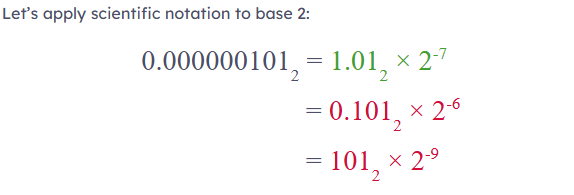
\includegraphics[width=0.5\linewidth]{二进制的科学计数法.png}
    \caption{二进制的科学计数法}
    \label{fig:enter-label}
\end{figure}
\textbf{溢出问题引导出偏移量表示法,又是一个基于前面的拓展}溢出主要有三种情况:上溢,下溢以及分数。我们用偏移量表示法就好,我们先确定一个偏移量然后把这个作为原点向两边拓展就是范围,取值也是二进制转化后加上偏移量优点:对不以原点为中心的情况非常合适。缺点:计算起来较为复杂\par
\textit{The 4 different representations have their own benefits and uses}\par
Unsigned无符号\par
Sign and Magnitude: has most problems有符号位\par
Bias notation偏移表示法\par
Two’s complement: most widely used implementation for signed integers二进制补码\par
\subsection{浮点数的表示规范IEEE介绍}
\begin{figure}
    \centering
    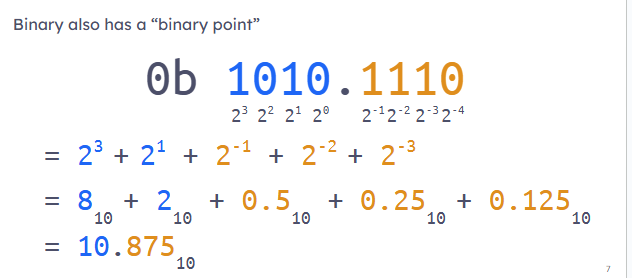
\includegraphics[width=0.25\linewidth]{image.png}
    \caption{关于二进制也有小数点的知识补充}
    \label{fig:enter-label}
\end{figure}
\subsubsection{IEEE基本格式}
\textbf{IEEE是浮点数的标准表示方法}
\begin{figure}
    \centering
    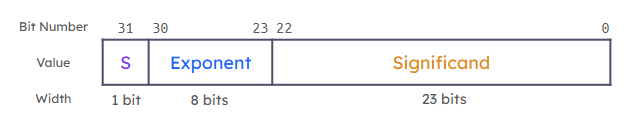
\includegraphics[width=0.25\linewidth]{浮点数格式.png}
    \caption{浮点数格式}
    \label{fig:enter-label}
\end{figure}
S区是符号区。
指数区:在偏置为 -127 的偏置表示法中
这意味着指数域 - 127 = 指数值,也就是说表示-128到127的指数区间。优点:
使具有相同符号的数字易于排序
在两个符号相同的浮点数之间,整数比较即可适用
value = $(-1)^(sign bit)*(1+Signficand)*2^(Exponent-127)$
\begin{figure}
    \centering
    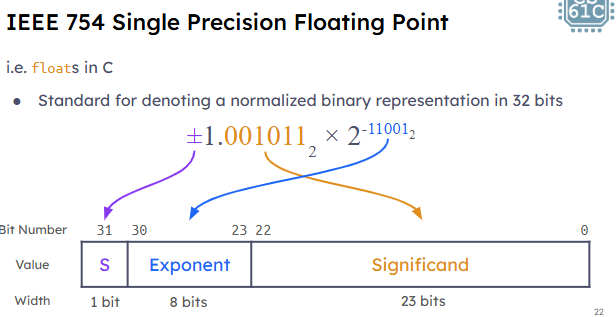
\includegraphics[width=0.5\linewidth]{ieee的一个例子.png}
    \caption{ieee的一个例子}
    \label{fig:enter-label}
\end{figure}
\subsubsection{IEEE中不同区域状态表示不同种类的数字}
\begin{figure}
    \centering
    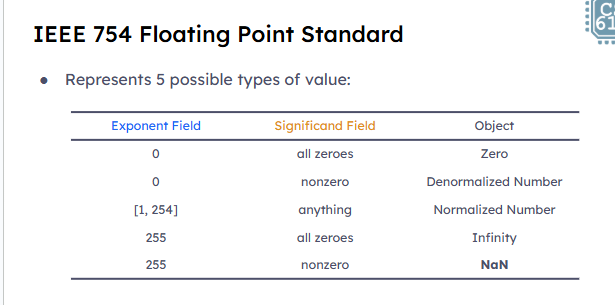
\includegraphics[width=0.5\linewidth]{各种情况展示.png}
    \caption{情况展示}
    \label{fig:enter-label}
\end{figure}对overflow和denormalized numbers记住指数区是偏移量,denormalized numbers表示了,无穷根据符号位分成正无穷和负无穷
有些数学运算完全无法得出有意义的结果,例如:
计算 
−4.0
​
 
(对 -4.0 开平方)
计算 
0.0/0.0
(0.0 除以 0.0)
然而,我们不想抛出错误。相反,我们有 “非数”(Not a Number)—— NaN。
它们用全为 1 的指数和非零的尾数来表示。例如:
0 1111 1111 0000 0000 0000 0000 0000 001=NaN\par
在 IEEE 754 标准中,非规格化数(Denormalized Numbers) 是一种特殊的浮点数表示形式,用于处理非常接近于零的数值,其特点和相关内容如下:1. 定义与表示形式当浮点数的指数位全为 0,且尾数部分不全为 0时,该数为非规格化数。与规格化数不同,非规格化数没有隐含的前导 1。规格化数的尾数隐含为 \(1.xxxx\)(二进制),而非规格化数的尾数为 \(0.xxxx\)(二进制)。2. 指数处理规格化数的指数采用偏置表示(如单精度偏置为 127,双精度偏置为 1023),而非规格化数的指数偏置为 126(单精度) 或 1022(双精度)。因此,非规格化数的实际指数值为 \(0 - 126 = -126\)(单精度)或 \(0 - 1022 = -1022\)(双精度)。3. 作用非规格化数用于填补下溢区域,使浮点数能表示比最小规格化数更小、更接近零的数值,增强了数值表示的连续性。例如,单精度非规格化数的取值范围为 \(\pm 0.f \times 2^{-126}\)(f 为 23 位尾数),双精度非规格化数为 \(\pm 0.f \times 2^{-1022}\)(f 为 52 位尾数)。4. 与规格化数的区别特性规格化数非规格化数指数位不全为 0 且不全为 1全为 0隐含前导 1有(尾数为 \(1.xxxx\))无(尾数为 \(0.xxxx\))指数偏置127(单精度)、1023(双精度)126(单精度)、1022(双精度)5. 注意事项非规格化数的运算可能影响性能。部分硬件对其支持不佳,需软件模拟,速度较慢;即使硬件支持,也可能比规格化数操作慢很多(如现代处理器上,规格化操作可能比非规格化快 100 倍)。非规格化数的引入减少了下溢异常,但可能增加除以 0 错误或 NaN(非数)出现的概率。总之,非规格化数是 IEEE 754 标准中处理极小数值的重要机制,通过特殊的指数和尾数表示,扩展了浮点数的表示范围,确保数值计算在接近零区域的平滑过渡。\par

 步长  
- 浮点数的步长是它与下一个最小浮点数之间的差值。  
- 这是有限尾数位数的结果。  
- 如何计算步长?  
    - 尾数最低有效位(LSB)的值。  
    - 对于规格化数:  
        步长 \( = 2^{(\text{指数域值} - 127 - 23)} \)(127 是单精度浮点数指数的偏置,23 是单精度尾数的位数,此公式基于单精度浮点数的规则)。  
    - 对于非规格化数:  
        步长 \( = 2^{(-126 - 23)} \)(-126 是单精度非规格化数的指数偏置,23 是单精度尾数的位数,此公式基于单精度浮点数的规则)。  

**讲解**:步长反映了浮点数能表示的最小精度间隔。由于尾数位数有限,相邻浮点数间存在固定差值。规格化数通过指数域值和固定参数计算步长,非规格化数因指数固定为特殊值(单精度下为 -126),步长计算也有特定形式。这种设计体现了浮点数在表示范围和精度上的权衡,有限的尾数位数决定了步长,也限制了浮点数能精确表示的数值间隔。 

\section{C的内存安排设置}
\textbf{这个的设置感觉想是作为最顶层开始从语言里面的内存安排,与下面的汇编语言感觉是一个作用}\par
\subsubsection{C的四个内存区介绍}
C的内存主要分为四个部分:栈:储存传递的函数参数和局部变量,从上到下延伸。当调用一个函数时,会分配一个栈帧。
这个栈帧包含以下内容:
返回地址(即函数执行完毕后要返回的位置),
函数的参数,用于存储局部变量的空间,
当函数返回时,该栈帧会被删除。使用时的危险点:指针在一个方向(调用者向被调用者)传入栈中是可行的。
而在另一个方向(被调用者向调用者)则是危险的\par
堆:是内存分配函数分配的区域,从下到上。
是动态的。
在运行时可以进行分配、调整大小和释放操作。
你需要使用堆来确保函数返回后指针仍然有效。
注意:堆是大量错误的根源。
(堆的使用)类似于 Java 中的 new 关键字 。
在 C 语言中,使用堆空间时要指定字节数:
malloc():分配的内存中包含随机数据(垃圾数据)。
calloc():分配的内存中只包含零值。
free():释放内存。
realloc():将内存大小调整为不同的尺寸(变大或变小)。
\subsubsection{堆的错误状况}
(堆内存)不会自动清理!作为程序员,你在使用完堆内存后必须显式地释放它。堆有四大易产生的bug:“Memory leak” — forgetting to free\par
“Use after free” — use a pointer that has been freed\par
“Double free” — Calling free 2x on the same memory\par
“Realloc can move stuff” — Forgetting this\par
\subsubsection{堆的内存分配函数}
void *malloc(sizet n)`
分配一块未初始化的内存。
- **参数**:一个参数,以字节为单位指定内存块的大小。
- **返回值**:返回 `void*` 类型。可以把它看作是指向任意类型的指针,后续课程会进一步讲解。若分配失败,返回 `NULL`。\par

void free(void* ptr)`
释放一块堆内存。
- **参数**:一个参数,即由 `malloc`、`realloc`、`calloc` 返回的原始指针。
- **注意事项**:确保在使用完每一块已分配的内存后都将其释放,否则会导致内存泄漏。\par

void *realloc(void* ptr, sizet size)`
改变已分配内存块的大小(增大或减小)。
- **返回值**:返回内存块的新地址,地址有可能已经发生了移动。
    - **常见做法**:`ptr = realloc(ptr, NEWSIZE)` 。
    - **更安全做法**:
        1. `TYPE *tmp = realloc(ptr, NEWSIZE);`
        2. `if (tmp) { ptr = tmp; }`
- **特殊情况**:
    - `realloc(NULL, size);` :行为类似于 `malloc` 。
    - `realloc(ptr, 0);` :行为类似于 `free` 。\par

void *calloc(sizet num, sizet size)`
分配一块初始化为零的内存。
- **内存大小**:新分配的内存大小为 `num * size` 字节。
- **示例**:`cardt *ret = calloc(1, sizeof *ret);`
- **注意**:如果 `size` 等于 `0` ,行为是未定义的。 \par
数据区:全局变量以及字符串字面量,还有大小是固定的\par
文本区:村塾可以执行的程序,也不会改变大小。
\begin{figure}
    \centering
    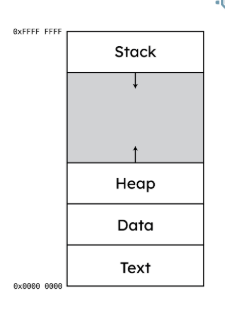
\includegraphics[width=0.5\linewidth]{c memory.png}
    \caption{C内存图}
    \label{fig:enter-label}
\end{figure}
\section{RISC-V}
\subsection{一个简单的对RISC-V介绍}
\textbf{现在开始介绍汇编语言的指令了,汇编语言作为机器码上面一层,感觉处在抽象的语言层和机器层的中间作为一个桥梁的作用}
\begin{figure}
    \centering
    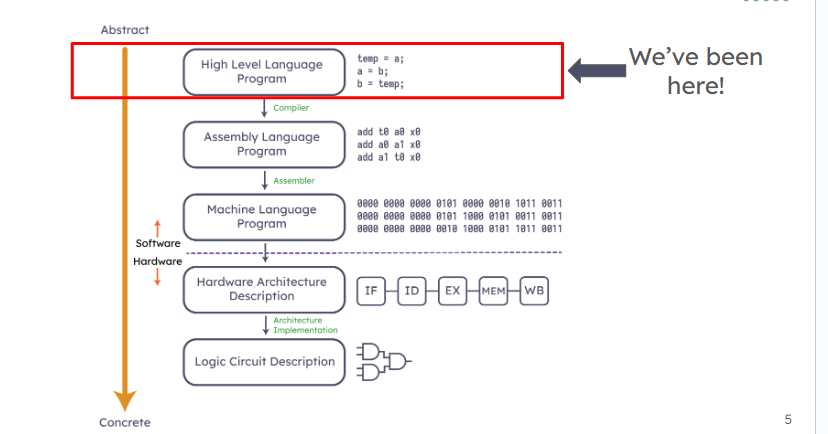
\includegraphics[width=0.5\linewidth]{目前的抽象.png}
    \caption{一张很好的关于我们目前学习的抽象状况的图}
    \label{fig:enter-label}
\end{figure}
电路一旦构建完成就很难更改。
相反,构建一个能够运行一组基础操作的电路,当这些操作组合在一起时,几乎可以描述任何行为 —— 这就是中央处理器(CPU)。
不同的 CPU 实现不同的操作集(也称为指令) —— 这被称为指令集架构(ISA)。
由 ISA 定义的编程语言被称为汇编语言。\par
相对于C来说,写汇编语言我们少了哪些便利: 允许你在一行代码中编写一系列操作,然后为你分解。
C 为你设置栈,并跟踪局部变量的存储位置。
C 允许你调用函数,并使用不会覆盖现有变量的局部变量。
C 允许你给变量命名,并跟踪该名称,甚至该名称所指变量的类型。\par
使用汇编语言时,几乎所有事情都由程序员显式处理。
\subsection{RISC-V的寄存器部分}

\begin{figure}
    \centering
    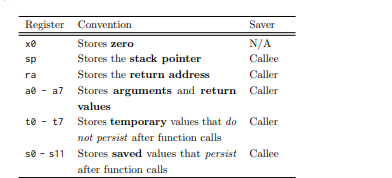
\includegraphics[width=0.5\linewidth]{寄存器规定.png}
    \caption{寄存器规定}
    \label{fig:enter-label}
\end{figure}


一个RISC - V系统由两个主要部分组成:  
- CPU,负责计算;  
- 主存储器,负责长期数据存储。  \par

CPU被设计得极其快速,通常每纳秒完成多条指令。访问主存储器通常需要数百甚至数千纳秒。  \par

CPU可以通过称为寄存器的组件存储少量数据。寄存器是一种被设计用于存储少量数据的CPU组件。每个寄存器存储32位数据(对于32位系统)或64位数据(对于64位系统)。在本课程中,我们只使用32位。寄存器的大小和数量是固定的(你可以认为它们是由硬件实现的)。 \par
\begin{figure}
    \centering
    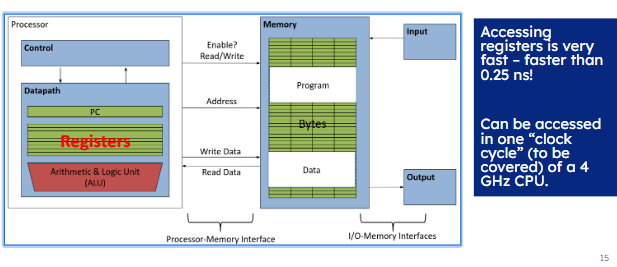
\includegraphics[width=0.5\linewidth]{描述CPU和内存在执行指令是的内部状态.png}
    \caption{描述CPU和内存器执行指令时的内部状态的一张好图}
    \label{fig:enter-label}
\end{figure}
\begin{figure}
    \centering
    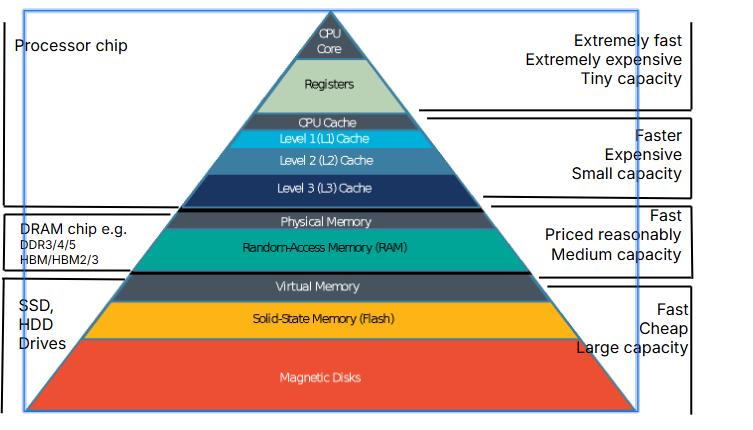
\includegraphics[width=0.5\linewidth]{不同硬件执行速度和容量的关系图.png}
    \caption{不同硬件执行速度和容量的关系图,相信我们以后还有不少机会见他}
    \label{fig:enter-label}
\end{figure}
RISC-V 提供了对 32 个寄存器的访问权限
寄存器编号从 0 到 31
通过编号引用:x0 – x31\par
寄存器 x0 是特殊的,它始终存储 0(尝试向该寄存器写入数据会被忽略)。因此,我们有 31 个寄存器可用于数据存储\par
其他 31 个寄存器的行为完全相同;不同寄存器之间的唯一区别是我们使用它们时遵循的约定。
\subsection{RISC-V的指令部分}
指令格式:每条 RISC-V 代码行都是一条单条指令,它对寄存器执行一个简单操作。\par
在 RISC-V 中,数据流向的操作数顺序是 “目标寄存器在左,源操作数在右”,逻辑上表现为从右(源)到左(目标)的流向,且这一规则在基础指令集中始终成立。这是 RISC-V 指令集设计的核心规范之一,确保了指令的简洁性和一致性
\subsubsection{算术操作符部分}




用于在寄存器之间或寄存器与立即数之间进行数学运算。以下操作在基础RISC - V指令集中可用:  \par
- 加法/减法:`add`(加)、`sub`(减)、`addi`(立即数加)\par  
- 按位运算:`and`(与)、`or`(或)、`xor`(异或)、`andi`(立即数与)、`ori`(立即数或)、`xori`(立即数异或)  \par
- 移位:`sll`(逻辑左移)、`srl`(逻辑右移)、`sra`(算术右移)\、`slli`(立即数逻辑左移)、`srli`(立即数逻辑右移)、`srai`(立即数算术右移)  \par
- 设置小于:`slt`(有符号小于)、`sltu`(无符号小于)、`slti`(立即数有符号小于)、`sltiu`(立即数无符号小于) \par
关于 “设置小于” 的说明:\par
slt x5 x6 x7 表示:如果 x6 < x7,则将 x5 设置为 1。否则,将 x5 设置为 0。\par
有两种版本:
slt(将操作数视为有符号数)
sltu(将操作数视为无符号数)
slti 和 sltiu 类似,但使用立即数代替 x7。
注意:乘法 / 除法不在基本指令集中,而是有一个可选的扩展。
注意无符号数来说,逻辑左移和逻辑右移与乘或除2的n次方等价,记住对于有符号数我们才用的是符号拓展,用最高位填充右移造成的空位\par
\subsubsection{A-FORMAT加法指令}
\begin{figure}
    \centering
    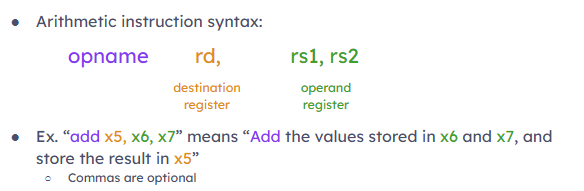
\includegraphics[width=0.25\linewidth]{加法指令格式.png}
    \caption{Enter Caption}
    \label{fig:enter-label}
\end{figure},对于减法指令,其实就相当于加取负后的那个值
这里数据从右向左流
伪指令\par
减少指令数量 → 减少 CPU 所需的电路。\par
有些命令可以用其他指令来编写,但我们希望有简写形式。\par
创建 “伪”(假)指令,这些指令在软件中会被转换为常规汇编指令\par
立即数版本:立即数是常数,对立即数参与的指令我们有特殊的版本:\par
add immediate:\par
\ \ \ \ \ \ \ \ \ \ \ addi \ x3, \ x4, \ 10\par
sub指令没有对于的立即数版本,直接对立即数取反就好,原因:将可执行的操作类型限制到绝对最少。
如果一个操作可以分解成更简单的操作,就不包含它。\par
加法中x0寄存器作用很大:零寄存器(x0)被硬编码为值 0;例如,add x3, x4, x0 等同于(在 C 语言中)f = g,其中 RISC - V 寄存器 x3、x4 与 C 变量 f、g 相关联。它在硬件中定义,所以一条add x0, x3, x4指令不会执行任何操作\par
\subsubsection{M-FORMAT内存指令格式}\par
\begin{figure}
    \centering
    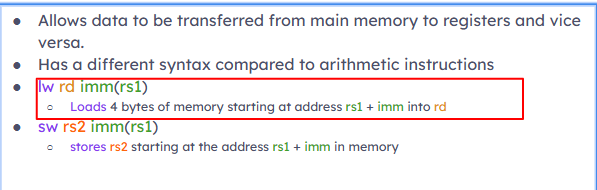
\includegraphics[width=0.25\linewidth]{内存指令格式示例.png}
    \caption{内存指令格式示例}
    \label{fig:enter-label}
\end{figure}
注意这里sw指令数据流向从左至右,但这因为左边读取右边寄存器中的地址再把左边寄存器数据存到内存上,而数据流向主要是指寄存器之间的,这个在寄存器之间遵守了规定,没有违反规律\par
这里的立即数单位都是字节,因为必须保证内存对齐\par
除了按字读取之外,还有按字节读取和存储的方式。lb,sb这种,这两个就是lw和sw的字节版本。读取寄存器的低八位也就是最低一个字节进行存储以及把值存进低八位再符号拓展\par
\subsubsection{C-FORMAT控制指令格式示例}\par
通常,在运行 RISC - V 代码时,我们总是按顺序执行下一行代码。\par
而控制指令则用于指定接下来要执行的不同代码行\par。控制指令有两种类型:
条件跳转(也称为分支):只有在满足特定条件时才会跳转到指定的代码行,否则继续执行下一行代码,这类似于 C 语言里的 if 语句。\par
无条件跳转:无论何种情况,都会跳转到指定的代码行。\par
标标签:用于特定代码行的便于人们阅读的标识符。\par
例如:\par
addi x5 x0 0 (将寄存器 x5 赋值为 0)\par
addi x6 x0 10 (将寄存器 x6 赋值为 10)\par
Loop: add x5 x5 x6 (标签 Loop,将 x5 与 x6 相加,结果存回 x5)\par
addi x5 x5 -1 (x5 的值减 1)\par
bne x5 x0 Loop (若 x5 与 x0 不相等,则跳转到标签 Loop 处)\par
条件跳转\par
分支类型
beq:如果两个寄存器值相等则分支 \par
bne:如果不相等则分支 \par
blt,bltu:如果小于(包括无符号变体)则分支 \par
bge,bgeu:如果大于或等于(包括无符号变体)则分支 \par
注意:bgt 不是一条指令,因为如果我们想执行 bgt x5 x6 Label,我们可以改用 blt x6 x5 Label。 \par
分支
格式:操作数 rs1 rs2 标签 \par
比较\textbf{从左到右}进行 \par
例如:beq x10 x11 somelabel \pare
如果 x10 等于 x11 则分支到 somelabel \par
例如:blt x20 x21 somelabel \par
如果 x10 小于 x11 则分支到 somelabel \par
无条件跳转:\par
两种形式:
跳转到标签\par
跳转到寄存器中保存的地址。\par
这些指令还会参考当前程序计数器(或称 PC),该计数器存储着当前正在运行的代码行的地址。
\par  
含义:将 x1 设置为 PC+4(即当前行的下一行代码地址),然后跳转到标签处。\par
伪指令说明
j 标签:这是一种简化的跳转指令,不进行链接操作。
jalr 目标寄存器 源寄存器 立即数:这是 “跳转并链接到寄存器指定地址” 指令的通用形式。
示例指令解释
jalr x1 x5 0(跳转并链接到寄存器指定地址):含义是将 x1 寄存器的值设置为当前程序计数器(PC)的值加 4(即下一条指令的地址),然后跳转到地址为 x5 + 0 处的代码行继续执行。
当我们不需要进行链接操作时,还会用到如下伪指令。
jr x1:跳转到寄存器 x1 所保存地址处的代码行继续执行,此过程不保存返回地址(即不进行链接操作)不保存返回地址其实就是把x0作为接受处
\begin{figure}
    \centering
    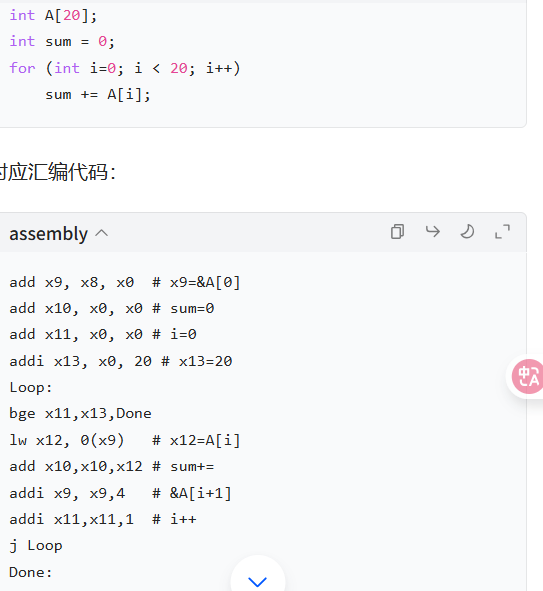
\includegraphics[width=0.5\linewidth]{1.png}
    \caption{一段很经典的C语言变汇编示例}
    \label{fig:enter-label}
\end{figure}
一条拓展指令:mul x5 x6 x7:将寄存器 x6 和 x7 中的值相乘,并将结果存储在寄存器 x5 中。
\subsubsection{RISC-V中的内存管理}
stack在ROSC-V中需要我们自己管理了,寄存器 x2 是栈指针(sp),被定义为指向栈底。 在函数开始时……
栈指针(sp)以上的数据被视为不可变的。
未经允许,你不得修改栈指针以上的任何内容。
栈指针以下的数据被视为可变的。
函数可以修改栈指针以下的任何内容。
但其他函数也可以修改它,所以你不能把数据留在那里并期望它保持不变。
在函数执行期间,我们可以通过递减栈指针在栈上分配空间。
但在函数调用结束后,栈指针必须恢复到函数调用前的值。 \par
\begin{figure}
    \centering
    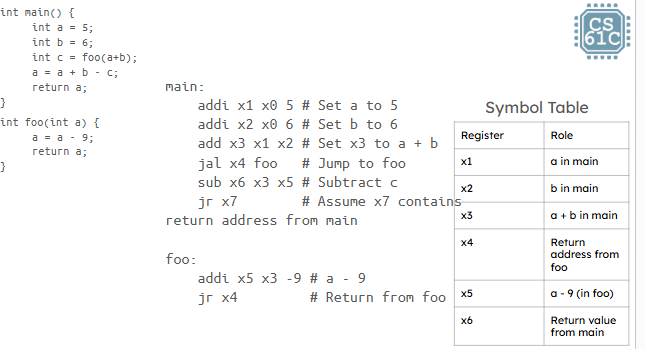
\includegraphics[width=0.5\linewidth]{一个简单的C语言翻译成RISCV的示例.png}
    \caption{一个简单的C语言翻译成RISCV的示例}
    \label{fig:enter-label}
    \end{figure}
    主要函数调用时记得jal以及jr的配套使用\par
    每个寄存器都会根据其作用被赋予一个名称(无需记住具体的对应关系):
zero:即 x0 寄存器,它始终存储值 0。\par
ra:即 x1 寄存器,用于存储返回地址。
(有两条新的伪指令会明确使用这个寄存器:
jal 标签 会被转换为 jal ra 标签
ret 会被转换为 jr ra)\par
被调用者保存寄存器:在函数调用结束前必须恢复原值的寄存器(即若要使用这些寄存器,被调用函数需保存其旧值)\par
sp:即 x2 寄存器,用作栈指针.\par
s0-s11:保存寄存器(用于存储需要保留的值).\par
\begin{figure}
    \centering
    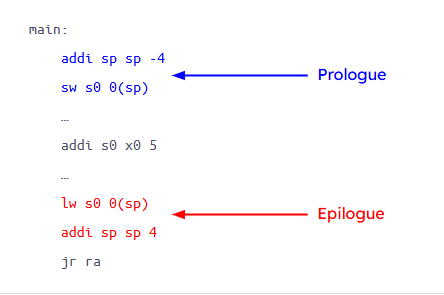
\includegraphics[width=0.5\linewidth]{使用堆保存.png}
    \caption{使用堆保存}
    \label{fig:enter-label}
\end{figure}

### 调用者保存寄存器:  
无需被调用函数恢复的寄存器(即若要在这些寄存器中保存变量,需在调用其他函数前将其值保存到某处)  
- `ra`:返回地址寄存器  
- `a0-a7`:用于传递函数参数的寄存器  
  - `a0`、`a1` 同时用于存放函数返回值  
  - 若函数参数超过 8 个,、\par
  用栈来存储额外参数  
- `t0-t6`:临时寄存器(用于临时存储中间结果,无需保留原值)\par这些寄存器超出作用域(不要使用它们)!
gp:即 x3 寄存器,用于存储对堆的引用,也称为 “全局指针”。
tp:即 x4 寄存器,用于存储线程的独立栈(多线程将在第 7 周讲解)。\par
调用函数时需要保存ra是因为防止嵌套调用导致值丢失:在函数调用过程中,`ra`(返回地址寄存器)的值是会发生变化的,下面详细解释为什么需要在函数调用结束后恢复 `ra` 的值。

### `ra` 寄存器的作用
在 RISC - V 架构里,`ra` 寄存器(也就是 `x1` 寄存器)专门用于存放返回地址。当使用 `jal`(跳转并链接)或者 `jalr`(跳转并链接到寄存器指定地址)这类指令调用函数时,`ra` 会被设置成调用指令之后紧接着的那条指令的地址。这样一来,在被调用的函数执行完毕后,就能够利用 `jr ra` 或者 `ret` 指令返回到调用函数的下一条指令处继续执行。

### 函数调用过程中 `ra` 值的变化
假设存在如下的汇编代码片段:
```assembly
main:
    addi t0, x0, 8
    addi sp, sp, -8
    sw t0, 0(sp)
    sw ra, 4(sp)
    jal ra, foo
    lw t0, 0(sp)
    lw ra, 4(sp)
    addi sp, sp, 8
    addi t0, t0, 3
     ...

foo:
     函数 foo 的具体实现
     可能会再次调用其他函数
    jal ra, bar
     ...
    ret
```
在 `main` 函数里,`jal ra, foo` 指令会把 `ra` 设置为 `lw t0, 0(sp)` 这条指令的地址,接着跳转到 `foo` 函数去执行。

要是 `foo` 函数又调用了别的函数(例如 `bar` 函数),`jal ra, bar` 指令会把 `ra` 设置为调用 `bar` 函数之后紧接着的那条指令的地址,这就会覆盖掉 `ra` 原本保存的返回 `main` 函数的地址。
\par
 恢复 `ra` 值的必要性\par
为了保证在 `foo` 函数执行完毕之后能够正确返回到 `main` 函数中调用 `foo` 之后的下一条指令处继续执行,就需要在调用 `foo` 函数之前把 `ra` 的值保存到栈上(`sw ra, 4(sp)`),在 `foo` 函数执行完毕返回之后再从栈上恢复 `ra` 的值(`lw ra, 4(sp)`)。

总结来说,在函数调用过程中,`ra` 的值会因为嵌套调用其他函数而发生改变,所以必须在函数调用前后保存和恢复 `ra` 的值,以此确保程序能够正确返回。 \par
\subsubsection{指令格式介绍}
对于 RV32(本课程所使用的版本)
不同的指令需要不同的值。
“add” 指定 3 个寄存器输入。
“addi” 指定 2 个寄存器和 1 个立即数。
思路:对不同的指令进行不同的编码。
整体设计理念:将格式相似的指令分类成组。对于每一组,定义 32 位如何用于保存所有需要的值。这称为指令格式。
尽可能使不同的格式相似!\par
 寄存器编号与识别\par
每个寄存器通过其编号来识别。由于总共有 32 个寄存器,所以需要 5 位二进制数就能唯一确定一个寄存器。例如:
 - `x0` 对应的二进制编号是 `0b00000`。
 - `a0` 也就是 `x10`,对应的二进制编号是 `0b01010`。\par

 指令各字段含义\par
- **`rd`(目标寄存器)**:用于存放指令运算结果的寄存器。\par
- **`rs1`(第一个源寄存器)**:为指令提供第一个操作数的寄存器。\par
- **`rs2`(第二个源寄存器)**:为指令提供第二个操作数的寄存器。\par
- **`opcode`(操作码)**:是指令的标识符,在所有指令格式中,它都位于指令的最后 7 位。某些相似的指令集合会被分配相同的操作码。例如,所有算术 R 类型指令的操作码都是 `0x33`。通常,具有相同格式的指令往往拥有相似的操作码。\par
- **`funct3`**:这是一个 3 位的标识符,用于区分操作码相同的不同指令。\par
- **`funct7`**:这是一个额外的 7 位标识符,用于区分那些操作码和 `funct3` 都相同但仍有细微差异的指令,比如 `sra`(算术右移)和 `srl`(逻辑右移)。 \par
\subsubsection{R-type}
\begin{figure}
    \centering
    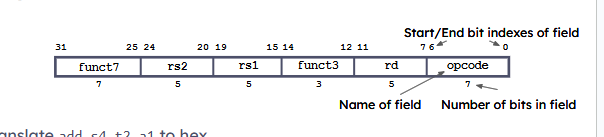
\includegraphics[width=0.5\linewidth]{Rtype.png}
    \caption{Enter Caption}
    \label{fig:enter-label}
\end{figure}
 R 类型指令格式介绍\par
这种指令格式专为涉及 3 个寄存器且无立即数的指令而设计,像 `add`(加法)或 `sub`(减法)这类算术运算符就使用此格式。\par
\begin{figure}
    \centering
    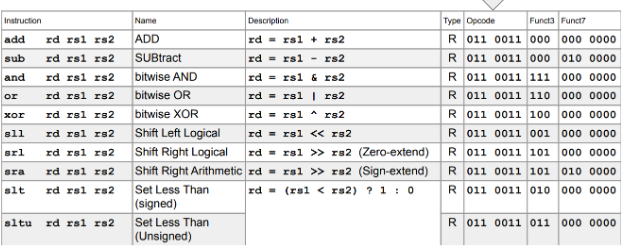
\includegraphics[width=0.5\linewidth]{R-type指令格式总结.png}
    \caption{R-type指令格式总结}
    \label{fig:enter-label}
\end{figure}
\subsubsection{I-type}
\begin{figure}
    \centering
    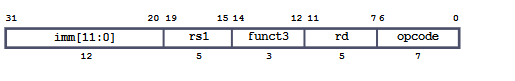
\includegraphics[width=0.5\linewidth]{I-type指令格式总结.png}
    \caption{I-type指令格式总结}
    \label{fig:enter-label}
\end{figure}
 I 类型指令格式介绍
I 类型指令格式专为包含 2 个寄存器(`rs1` 和 `rd`)以及 1 个立即数的指令而设计。适用的指令类型包括:
- **带立即数的算术运算指令**:如 `addi`(立即数加法)、`andi`(立即数按位与)、`slti`(立即数小于则置位)等。
- **加载指令**:像 `lw`(加载字)、`lh`(加载半字)、`lhu`(无符号加载半字)、`lb`(加载字节)、`lbu`(无符号加载字节)。
- **`jalr` 指令**:跳转并链接到寄存器指定地址。

需要注意的是,`ecall`(系统调用)和 `ebreak`(调试断点)技术上也属于 I 类型指令,但它们会忽略 `rd`、`rs1` 和立即数,这些字段的值在它们的使用场景中并无实际意义。而存储指令会用到 `rs1` 和 `rs2`,所以为其设计了单独的指令格式。

 指令各字段存储方式\par
I 类型指令的大部分组成部分与之前介绍的存储方式相同,只是新增了 `imm`(立即数)部分。立即数存储在 `imm` 组件中。特别要注意 `[11:0]` 这种表示方式,它意味着将立即数的第 11 位存放在指令的第 31 位位置,第 10 位存放在第 30 位位置,以此类推,第 0 位存放在第 20 位位置。\par

 I 类型立即数的特点\par
- **位数限制**:I 类型的立即数为 12 位。这就决定了我们只能将一个 12 位的整数作为立即数来存储。
- **数值范围**:大多数指令使用有符号立即数,所以 I 类型立即数的取值范围是 [-2048, 2047]。例如,“`addi sp sp -2048`” 是有效的 RISC - V 代码,而 “`addi sp sp -2052`” 则不是有效的代码。
- **移位指令特殊情况**:对于移位指令(如 `slli` 逻辑左移立即数、`srli` 逻辑右移立即数、`srai` 算术右移立即数),最大移位量为 31。因为任何更大的移位量都会使所有数据移出寄存器。这些移位指令属于修改后的 I 类型,会额外指定一个 `funct7` 字段。 \par
\begin{figure}
    \centering
    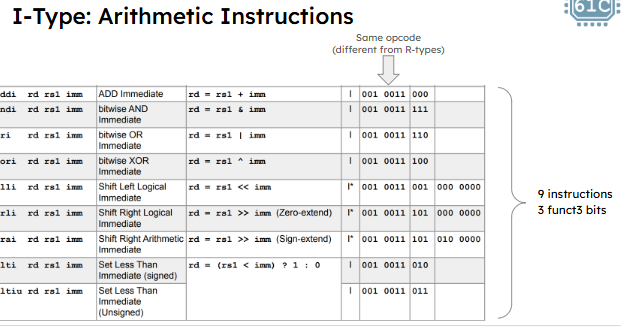
\includegraphics[width=0.5\linewidth]{I-type格式总结.png}
    \caption{I-type格式算术指令部分总结}
    \label{fig:enter-label}
\end{figure}
\begin{figure}
    \centering
    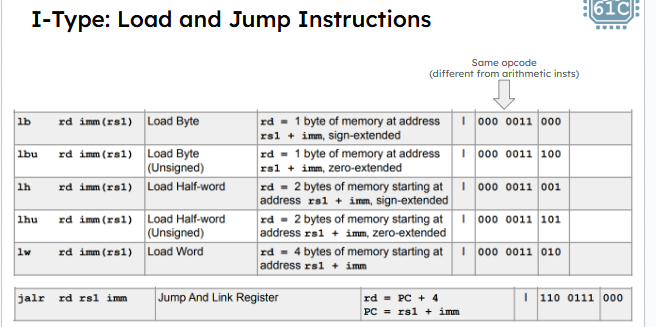
\includegraphics[width=0.5\linewidth]{I-type格式总结加载和跳转部分.png}
    \caption{I-type格式总结加载和跳转部分}
    \label{fig:enter-label}
\end{figure}
\subsubsection{S-type}
\begin{figure}
    \centering
    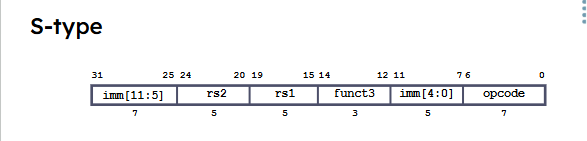
\includegraphics[width=0.5\linewidth]{S-type指令格式.png}
    \caption{S-type指令格式}
    \label{fig:enter-label}
\end{figure}
 S 类型指令格式介绍
这种指令格式专为包含 2 个源寄存器和 1 个立即数的指令而设计,主要用于存储指令。

 立即数拆分原因
在 S 类型指令中,立即数是被拆分存储的。这么做是为了让 `rs1` 和 `rs2` 寄存器的位置与 R 类型指令中的位置保持一致。通过这种方式,可以在不同指令格式之间维持一定的规律性,便于硬件设计和指令处理。

 立即数的存储方式
S 类型指令中的立即数存储方式与 I 类型有相似之处,但需要将立即数“拼接起来”。具体来说,立即数会被拆分成两部分,分别存放在指令的不同位置。

 示例说明
例如,如果有一个立即数为 `0b1101 0101 0001`,那么会把 `0b110 1010` 存放在第一个立即数存储位置,把 `0b10001` 存放在第二个立即数存储位置。这样,在指令执行时,硬件会将这两部分重新组合成完整的立即数来使用。 
\begin{figure}
    \centering
    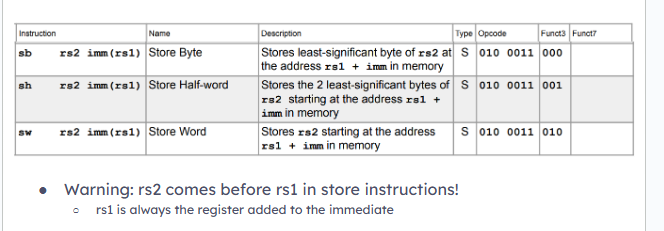
\includegraphics[width=0.5\linewidth]{S-type指令汇总.png}
    \caption{Enter Caption}
    \label{fig:enter-label}
\end{figure}
\subsubsection{U-type}
 1. `lui` 和 `auipc` 指令介绍
 `lui`(Load upper immediate)指令
`lui rd imm` 指令的作用是将立即数 `imm` 左移 12 位后的值存入目标寄存器 `rd`。例如 `lui t0 0x12345` 会让 `t0` 寄存器的值变为 `0x12345000`。

 `auipc`(Add upper immediate to Program Counter)指令
`auipc rd imm` 指令会把立即数 `imm` 左移 12 位后的值与程序计数器(PC)的值相加,结果存入目标寄存器 `rd`。

 2. 伪指令 `li` 和 `la` 的实现
`li` 和 `la` 是伪指令,它们依赖 `lui` 和 `auipc` 来实现具体功能:
 - `li rd imm`:将立即数 `imm` 存入寄存器 `rd`。
 - `la rd Label`:将标签 `Label` 的地址存入寄存器 `rd`。

 3. 大立即数的处理
当要把一个 32 位的立即数存入寄存器时,不能直接使用 `addi` 指令,因为 `addi` 指令的立即数只有 12 位。例如要实现 `li t0 0x12345678`,可以使用 `lui` 和 `addi` 组合:
```assembly
lui t0 0x12345
addi t0 t0 0x678
```
这里 `lui` 先将高 20 位存入 `t0`,`addi` 再将低 12 位加上去。

### 4. 负数立即数的处理
对于像 `li t0 0xABCDEFFF` 这样的情况,如果直接写成:
```assembly
lui t0 0xABCDE
addi t0 t0 0xFFF
```
会出现问题。因为 `addi` 的立即数是有符号的,`0xFFF` 会被解释为 -1。所以正确的做法是:
```assembly
lui t0 0xABCDF
addi t0 t0 -1
```
这样就能得到正确的结果 `0xABCDEFFF`。

 5. `auipc` 与相对寻址
#### 相对寻址的优势
在编写代码时,通常希望多个程序(如库)能够组合在一起,这可能会改变指令的地址。使用绝对地址(如 “这个标签位于地址 `0x000000FC`”)在标签地址改变时会出错,而相对地址(如 “这个标签在当前代码行之后 48 字节处”)在代码和标签一起移动相同距离时仍然有效。

`auipc` 与 `la` 的结合
`auipc` 常与 `la` 指令配合使用。`auipc` 通过将立即数左移 12 位后与 PC 相加,提供了一种基于当前指令位置的相对寻址方式,有助于在代码组合时避免地址问题。

综上所述,`lui` 和 `auipc` 指令在处理大立即数和实现相对寻址方面发挥着重要作用,使得 RISC - V 汇编语言能够更灵活地编写代码。 
\begin{figure}
    \centering
    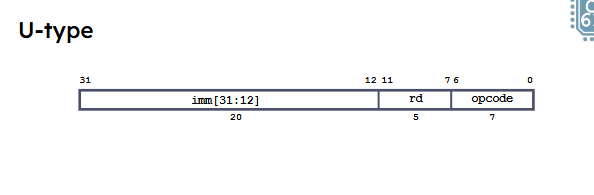
\includegraphics[width=0.5\linewidth]{U-type指令格式.png}
    \caption{U-type指令格式}
    \label{fig:enter-label}
\end{figure}、
\begin{figure}
        \centering
        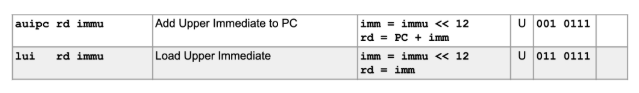
\includegraphics[width=0.5\linewidth]{U-type指令总结.png}
        \caption{U-type指令总结}
        \label{fig:enter-label}
    \end{figure}
    \subsubsection{B-type}
    在机器码里不存在标签。把 RISC - V 汇编代码转换为二进制代码时,要把所有标签都转换为对特定代码行的明确引用。\par

回顾一下:由于我们希望能够在内存中移动代码块,所以更倾向于使用相对寻址,而非绝对地址。\par

解决方案:在汇编使用了标签的代码时,首先要把标签转换为偏移量。这个偏移量指明了为到达该标签所指向的位置,需要跳转的字节数。 \par
\begin{figure}
    \centering
    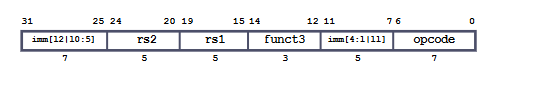
\includegraphics[width=0.5\linewidth]{B-type格式.png}
    \caption{B-type格式}
    \label{fig:enter-label}
\end{figure}
有两个源寄存器和一个立即数(类似于 S 类型指令)。
B 类型指令有时也被称为 SB 类型指令。
注意,立即数以一种奇特的模式存储。
这是为什么呢?
立即数的最高有效位(MSB)存于指令的最高有效位,这样做是为了简化符号扩展。
第 10 位到第 1 位在指令中的位置与 S 类型指令中相同。
我们能实现多远的跳转呢?
12 位加上 1 位,也就是 13 位的立即数,其范围是 [-4096, 4094],即最多可以向上或向下跳转 210 条指令的距离。
\begin{figure}
    \centering
    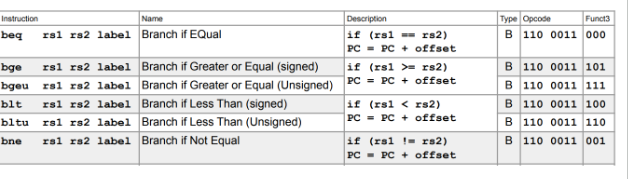
\includegraphics[width=0.5\linewidth]{B-type指令总结.png}
    \caption{B-type指令总结}
    \label{fig:enter-label}
\end{figure}
\subsubsection{J-type}
JAL(跳转并链接)指令仅使用一个目标寄存器和一个立即数,因此我们可以采用与 U 型指令类似的格式来获取额外的立即数位。J 型指令有时也被称为 UJ 型指令。需要注意的是,立即数以一种更为奇特的模式存储。要留意的是,我们把立即数的最高有效位(MSB)放在指令的最高有效位处,第 19 - 12 位与 U 型指令中的位置相同,第 10 - 1 位与 I 型指令中的位置相同。和之前一样,最低位不进行存储。20 位加上 1 位,即 21 位的立即数,所以最多可以向上或向下跳转 \(2^{18}\) 条指令的距离。
\begin{figure}
    \centering
    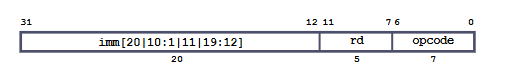
\includegraphics[width=0.5\linewidth]{J-type指令格式.png}
    \caption{J-type指令格式}
    \label{fig:enter-label}
\end{figure}
\begin{figure}
        \centering
        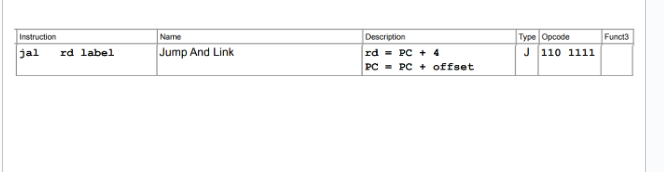
\includegraphics[width=0.5\linewidth]{J-type指令总结.png}
        \caption{J-type指令总结}
        \label{fig:enter-label}
    \end{figure}
    如何处理超出存储范围的立即数(第 1 部分,共 2 部分)R 型指令:
没有立即数。U 型指令:
用于处理这些立即数。I 型和 S 型指令:
对于算术指令,通常可以先将立即数存储到一个临时寄存器中。例如,如果我们想执行 xor t0 t1 0xDEADBEEF 操作,我们可以这样做:plaintextli t2 0xDEADBEEF
xor t0 t1 t2
对于加载和存储操作,我们可以先加上偏移量,然后进行零偏移加载(就像可变偏移加载那样)。B 型和 J 型指令:分支指令情况:如果分支目标在当前指令的 1024 条指令范围内?
正常进行分支操作(例如 beq t0 t1 Label)。如果分支目标超出当前指令的 1024 条指令范围?
反转分支条件,然后使用 j 指令代替:plaintextbne t0 t1 Next
j Label
Next:
跳转指令情况:如果跳转目标在当前指令的 \(2^{18}\) 条指令范围内?
正常进行跳转操作(例如 j Label)。如果跳转目标超出当前指令的 \(2^{18}\) 条指令范围?
先执行 auipc 指令,然后使用 jalr 指令的立即数来完成剩余的偏移:plaintextauipc t0 0x12345\par
jalr ra t0 0x678\par
\subsection{CALL}
\textbf{这节主要的内容是讲解CALL,一段C语言代码变成机器码的过程}
\begin{figure}
    \centering
    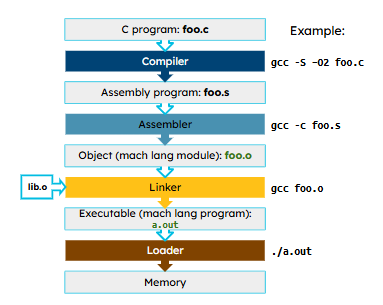
\includegraphics[width=0.5\linewidth]{CALL.png}
    \caption{CALL}
    \label{fig:enter-label}
\end{figure}
\begin{figure}
    \centering
    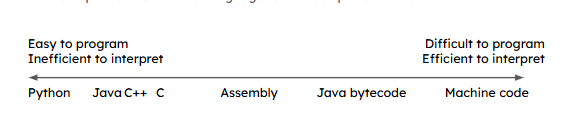
\includegraphics[width=0.5\linewidth]{语言的直接执行性能和翻译器效率.png}
    \caption{语言的直接执行性能和翻译器效率}
    \label{fig:enter-label}
\end{figure}
\subsubsection{预处理}
注意:预处理程序(Preprocessor)在编译器之前(大致)运行,并处理以下指令:
#define 语句(定义常量或宏)
#include 语句(包含头文件)
条件语句(#if、#endif、#ifdef、#else 等)
宏(对象 / 数据宏、函数宏等)
输出:纯 C 文件
\subsubsection{编译}
输入 / 输出:C 语言 / 低级语言 ⇒ RISC - V 汇编语言 / 其他汇编语言
在这个阶段会进行优化。
这是编译难度的瓶颈所在。
这可是 CS 164 课程的内容呢!(注:CS 164 可能是某所学校关于编译相关课程的编号)
输出结果将会包含:
标签
伪指令
\subsubsection{汇编}
### 翻译
输入/输出:优化后的 RISC - V 汇编代码(*.s)⇒ 目标文件(*.o)\par

目标文件包含以下内容:\par
- **文件头**:
    后续各组件的大小和位置信息。
- **文本段**:
    机器码。
- **数据段**:
    所有静态数据的二进制表示。
- **符号表**:
    填充有标签及其相对地址。
- **重定位表**:
    填充有需要定位的值(包括文件内部和外部的)。
- **调试信息**:
这些关键字(如 .text、.data、.globl、.string、.word 等)是汇编语言中的,出现在汇编语言源文件(通常以 .s 为扩展名)中。它们属于汇编语言中的伪指令(或汇编指示符),用于指导汇编器对代码和数据进行处理,虽不生成机器码,但对汇编过程至关重要\par
这些是某种类型的关键字,它们为汇编器提供指引,但不会生成任何机器指令(目标文件中的二进制输出)。\par
- **.text**:后续的项将被放入用户文本段(机器码)。\par
    这通常包含所有的代码,并且在大多数汇编文件中是最后一个段。
- **.data**:后续的项将被放入用户数据段(源文件数据的二进制形式)。\par
    这通常是源文件中静态和全局变量定义的地方。\par
- **.globl sym**:声明符号 `sym` 在多个文件中是全局的,并且可以从其他文件中引用。\par
- **.string str**:将字符串 `str` 存储在内存中,并以空字符结尾。\par
- **.word w1...wn**:将 n 个 32 位的量依次存储在连续的内存字中。\par

\textbf{符号表是别的或自己要跳转到这个里面用到的索引,重定位表是自己要跳到自己或别人那里面的索引}

\par
符号表  \par
- 此文件中可能被生成它的文件或其他文件使用的“项”的列表。  
- 本文件使用它来替换前向引用。  
  - 前向引用:在代码中定义之前就被指令使用的标签。  
- 其他文件使用它来替换它们自己的外部引用。  
  - 外部引用:被不在同一文件中定义的指令使用的标签。  
  - C 语言中的外部引用可能包括调用需要导入预定义 C 头文件或自定义定义的函数。  
    - #include <stdio.h>  
    - #include “yourown.h”  
- 符号表通常包含什么?  
  - 标签:函数调用。  
  -.data 段中的数据变量。  
\par
重定位表  \par
- 此文件需要其地址的“项”的列表,包括可能在本地或外部定义的标签。  
- 这些标签/项包括什么?  
  - 任何跳转到的绝对标签:jal, jalr。  
  - 有时是内部标签。  
  - 总是包括外部标签(包括库文件)。  
  - 当由 LUI 定义时的 la 指令。  
  - 静态段中的任何数据块。  
- 链接阶段使用的信息。 
\begin{figure}
    \centering
    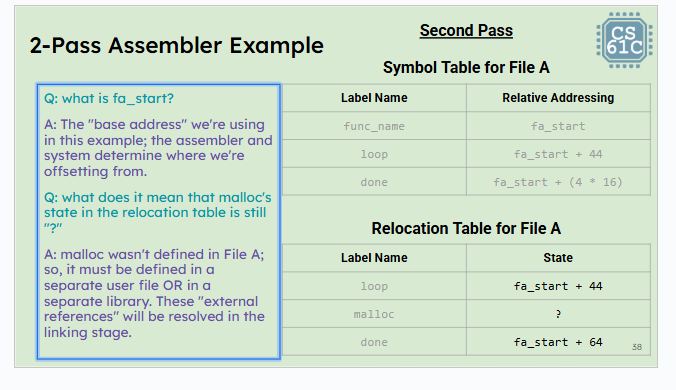
\includegraphics[width=0.5\linewidth]{简单的符号表和重定向表例子.png}
    \caption{简单的符号表和重定向表例子}
    \label{fig:enter-label}
\end{figure}
\begin{figure}
    \centering
    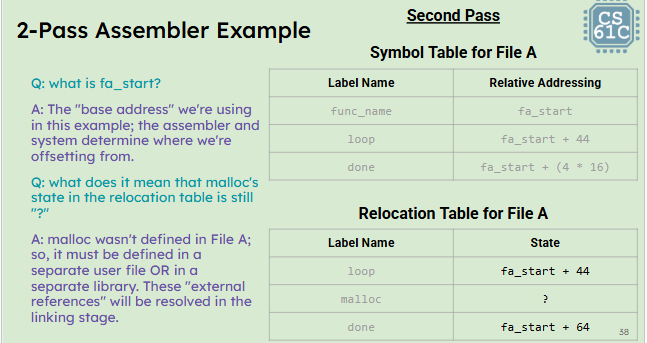
\includegraphics[width=0.5\linewidth]{关于上面的一点补充.png}
    \caption{关于上面的一点补充}
    \label{fig:enter-label}
\end{figure}
\begin{figure}
    \centering
    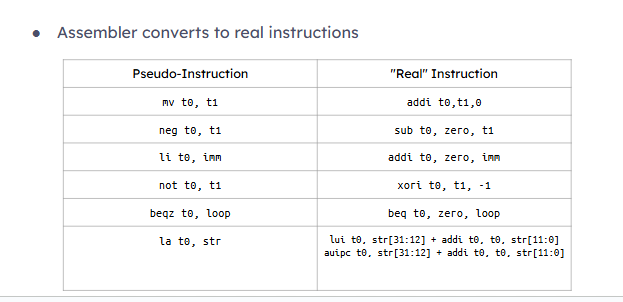
\includegraphics[width=0.5\linewidth]{汇编器对伪指令的替换.png}
    \caption{ 汇编器对伪指令的替换  }
    \label{fig:enter-label}
\end{figure}
\textbf{对于机器码的生成}\par
简单情况:算术、逻辑、移位等操作
指令本身已经包含了所有必要的信息。
那么,基于程序计数器(PC)的相对跳转(如 jal 指令)和分支(如 beq、bne 指令)呢?\par
通过计算目标位置与跳转指令之间的指令半字数量,来确定偏移量。
注意:需要先替换伪指令,才能知道分支或跳转所涉及的指令数量。
那么,对静态数据的引用呢?
“la” 指令有时可以拆分为 “lui” 和 “addi” 指令(对于基于 PC 的相对引用,使用 “auipc” 和 “addi”)。
这些操作需要获取数据的完整 32 位地址。
目前还无法确定这些地址,所以我们创建两个表格:
符号表和重定位表,让链接器来解决这些问题!
“前向引用” 问题
使用标签的指令可能会引用程序中 “位于后面” 的标签。
通过对程序进行两遍扫描来解决这个问题:
第一遍扫描记录标签的位置;
第二遍扫描利用标签的位置来生成代码。\par
\subsubsection{链接}
\begin{figure}
    \centering
    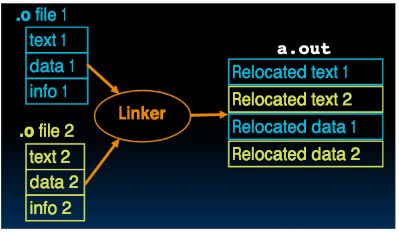
\includegraphics[width=0.5\linewidth]{链接可视化.png}
    \caption{链接可视化}
    \label{fig:enter-label}
\end{figure}
目标文件(.o) ⇒ 可执行文件(.out)
对每个目标文件中的代码块(段)进行分类,并按顺序将它们组合在一起。
顺序由链接器确定。
标准段包括:文本段、数据段。
解析所有引用:
对用户文件的引用 → 符号表
外部引用 → 静态 / 动态链接库文件
遍历所有重定位项。
结果:所有绝对地址都被填充。\par
具体:
步骤 1:从每个 .o 文件中取出文本段并将它们合并在一起。
步骤 2:从每个 .o 文件中取出数据段,将它们合并,并将其连接到文本段末尾。
步骤 3:解析引用
遍历重定位表,处理每个表项。
即填充所有绝对地址。.out 文件包含:
头部:记录文本段和数据段的大小。
为何不需要文本 / 数据段的位置?因为此时所有内容已合并在一起。\par
四种地址\par
PC 相对寻址(beq、bne、jal;auipc/addi):无需重定位(PIC:位置无关代码)。
绝对函数地址(auipc/jalr):始终需要重定位。
外部函数引用(auipc/jalr;jal extlabel):始终需要重定位。
静态数据引用(常用 lui/addi):始终需要重定位.\par
链接器假定在 RV32 架构中,第一个文本段的第一个字位于地址 0x10000(在 RV64 架构中为 0x40000000)。
链接器已知信息:
每个文本段和数据段的长度。
文本段和数据段的排列顺序。
链接器执行的计算:
计算每个要跳转的标签(内部或外部)以及每个被引用的数据块的绝对地址。
为解析引用:
在所有 “用户” 符号表中搜索引用(数据或标签)。
如果未找到,则搜索库文件(例如,查找 malloc 函数)。
一旦确定了绝对地址,就相应地填充机器码。\par
静态和动态链接库之间:\par
1. 链接时机与文件构成\par
静态链接库:在链接阶段,库代码会被完整地包含到可执行文件中,成为其一部分。例如,若程序使用了静态链接的数学库,最终可执行文件会携带该库的全部代码。
动态链接库:程序在运行时才会链接库。可执行文件仅包含对库的引用信息,而非库代码本身。如 Windows 下的 .dll 或 Linux 下的 .so 文件,程序运行时才加载这些库。\par
2. 空间占用\par
静态链接库:会增加可执行文件的体积。即使只使用库中的一个函数,也会包含整个库的代码,浪费磁盘空间。
动态链接库:
节省磁盘空间,多个程序可共享同一库文件,无需重复存储。
内存使用更高效,若多个程序共享一个库,只需加载一次库到内存,减少内存占用。\par
3. 更新与维护\par
静态链接库:若库更新(如修复漏洞或增加功能),使用该库的可执行文件必须重新编译链接才能享受更新,否则仍使用旧库代码。
动态链接库:只需更新库文件(如替换 libXYZ.so),所有使用该库的程序在运行时会自动链接新库,无需重新编译可执行文件。但这也带来依赖问题,若库文件被删除或版本不兼容,程序可能无法运行。\par
4. 移植性\par
静态链接库:可执行文件自包含,不依赖外部库,移植到其他环境(如另一台机器)时,只要目标系统支持程序运行的基本环境(如操作系统内核版本),即可直接运行,无需额外携带库文件。
动态链接库:可执行文件依赖外部库文件,移植时需确保目标环境有兼容的库文件,否则程序无法运行。\par
5. 运行效率\par
静态链接库:由于库代码已在可执行文件内,运行时无需额外的链接操作,函数调用直接执行,理论上速度稍快。
动态链接库:程序运行时需进行库的加载和链接,存在一定的时间开销。但现代操作系统对动态链接优化良好,这种开销通常较小。\par
\subsubsection{加载}
可执行文件(*.out)加载到内存:
为将文本段和数据段加载到内存空间做好必要的空间准备。
把文本段和数据段复制到这个内存空间中。
用程序参数初始化栈。
将栈指针设置在参数下方的最高位置。
把栈寄存器的值设为栈指针的地址。
清空大多数其他寄存器(将其值设为零)。
跳转到启动例程,该例程会把程序的参数从栈复制到寄存器中,并设置程序计数器(PC)。
程序计数器:这是一个专用寄存器,用于保存当前正在执行的代码行的内存地址。\par
\subsubsection{总结一下}
编译:它的实际含义是什么(并且发现这仅仅是一个漫长过程的第一步)。\par
汇编:汇编代码中便于人类阅读的部分是如何被替换为更便于机器识别的特征的。\par
链接:不同的文件和库是如何整合到最终产品中的。\par
加载:系统是如何处理我们的代码并使其得以运行的\par
\section{处理器单元构建}
\subsubsection{最简单的组合逻辑和有限状态机引入}
\begin{figure}
    \centering
    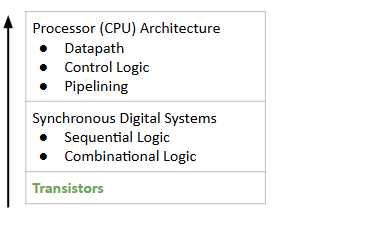
\includegraphics[width=0.5\linewidth]{从晶体管到cpu.png}
    \caption{从晶体管到cpu}
    \label{fig:enter-label}
\end{figure}

同步数字系统与 CPU 架构紧密相关,二者是基础与应用、底层与高层的关系,具体体现在以下方面:  \par

1. 同步数字系统是 CPU 架构的底层基础  \par
- **逻辑基础**:同步数字系统包含时序逻辑(Sequential Logic)和组合逻辑(Combinational Logic)。  
    - 组合逻辑用于实现即时的逻辑运算与数据处理,例如 CPU 架构中算术逻辑单元(ALU)对数据的加减乘除等操作,本质上依赖组合逻辑实现。  
    - 时序逻辑通过时钟信号协调系统操作,确保各部件按顺序工作。CPU 架构中的指令执行流水线、寄存器数据更新等,都需要在时钟同步下进行,以保证操作的时序正确性。  
- **同步机制**:同步数字系统通过统一的时钟信号实现各部件同步,这一机制是 CPU 架构正常运作的关键。例如,CPU 取指令、解码、执行等阶段的切换,都由时钟信号驱动,确保每个操作在准确的时间点执行,避免数据冲突与操作混乱。  \par

 2. CPU 架构是同步数字系统的高级应用与扩展  \par
- **功能实现**:CPU 架构中的数据通路(Datapath)、控制逻辑(Control Logic)、流水线(Pipelining)等设计,是对同步数字系统的具体应用。例如,数据通路中数据的流动与处理,依赖同步数字系统的逻辑门电路及时序控制;控制逻辑通过生成控制信号协调各部件,其底层实现基于组合逻辑与时序逻辑的协同工作。  
- **优化与扩展**:CPU 架构在同步数字系统基础上进行优化创新。如流水线技术将指令执行分为多个阶段,每个阶段在时钟驱动下并行处理不同指令,提升处理效率,这是对同步数字系统时序控制的扩展应用;现代 CPU 架构引入多级缓存(Cache),通过同步机制保证缓存与主存数据的一致性,也是对同步数字系统的灵活运用。  \par
\subsubsection{晶体管}
\begin{figure}
    \centering
    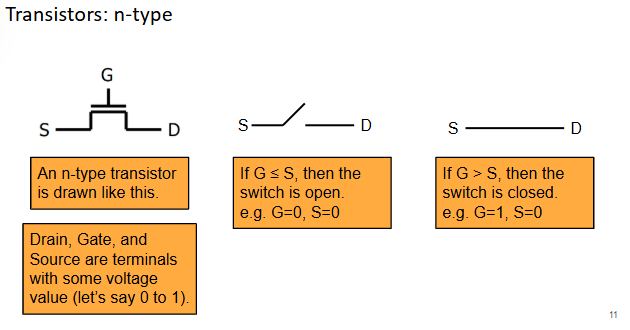
\includegraphics[width=0.5\linewidth]{n-type.png}
    \caption{n-type}
    \label{fig:enter-label}
\end{figure}
\begin{figure}
    \centering
    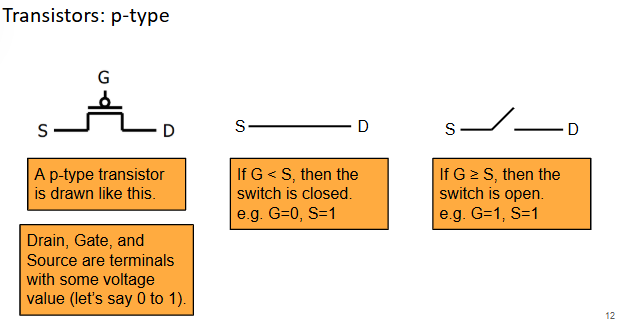
\includegraphics[width=0.5\linewidth]{p-type.png}
    \caption{p-type}
    \label{fig:enter-label}
\end{figure}
图示区分:p多了一个小圈
\begin{figure}
    \centering
    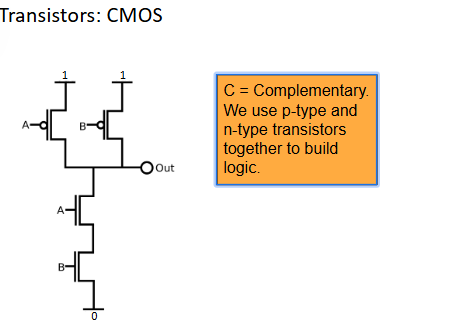
\includegraphics[width=0.5\linewidth]{使用着两种晶体管构建的逻辑电路示例.png}
    \caption{使用着两种晶体管构建的逻辑电路示例}
    \label{fig:enter-label}
\end{figure}
\subsubsection{逻辑门}
具有以下特性的运算符:\par
一个或多个 1 位输入,
一个 1 位输出,
可由晶体管构成,
可表示为:
电路图中的一个模块,
一个真值表(列出所有可能输入对应的输出),
一个布尔代数表达式,
用于执行按位运算,
\begin{figure}
    \centering
    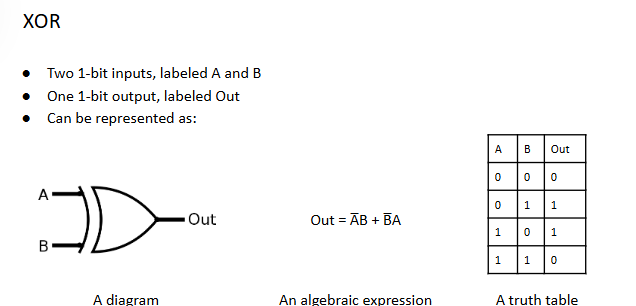
\includegraphics[width=0.5\linewidth]{xor.png}
    \caption{xor}
    \label{fig:enter-label}
\end{figure}
\begin{figure}
    \centering
    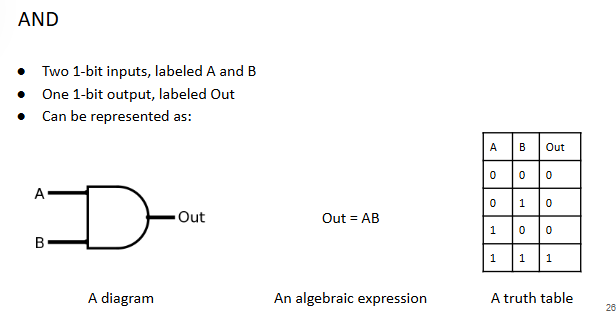
\includegraphics[width=0.5\linewidth]{and.png}
    \caption{and}
    \label{fig:enter-label}
\end{figure}
\begin{figure}
    \centering
    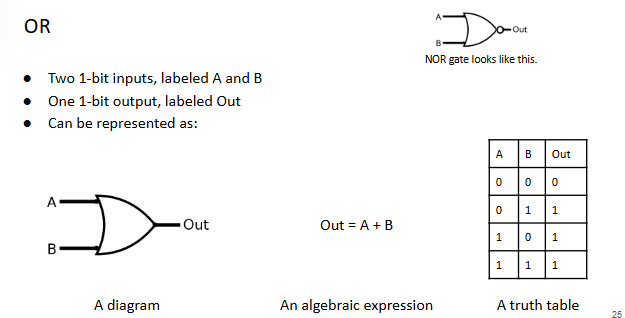
\includegraphics[width=0.5\linewidth]{or.png}
    \caption{or}
    \label{fig:enter-label}
\end{figure}
\begin{figure}
    \centering
    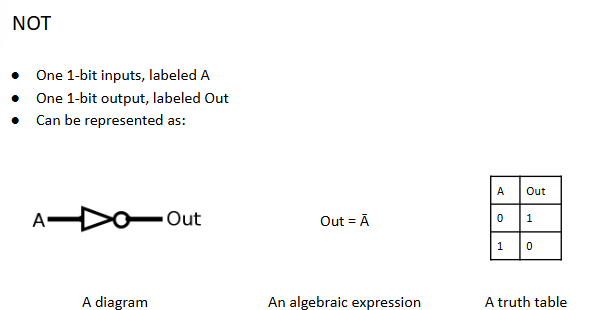
\includegraphics[width=0.5\linewidth]{not.png}
    \caption{Enter Caption}
    \label{fig:enter-label}
\end{figure}
\subsubsection{组合逻辑}
组合逻辑有点像纯函数,不受状态影响,如果不把状态看作一个输入的话\par
重要的一个技巧是根据真值表简化电路的表达式\par
\begin{figure}
    \centering
    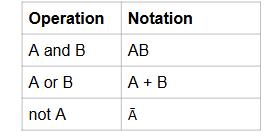
\includegraphics[width=0.5\linewidth]{语言中的逻辑操作在布尔表达式中的符号.png}
    \caption{语言中的逻辑操作在布尔表达式中的符号}
    \label{fig:enter-label}
\end{figure}
、
\begin{figure}
    \centering
    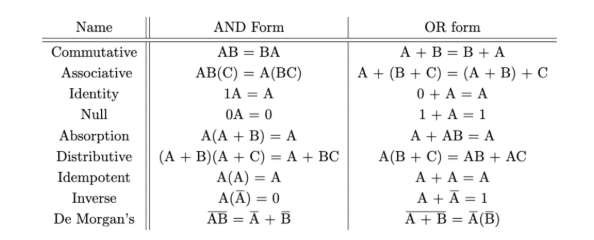
\includegraphics[width=0.5\linewidth]{布尔表达式的表.png}
    \caption{布尔表达式计算技巧的表}
    \label{fig:enter-label}
\end{figure}
给定一个真值表,我们如何将其转换为布尔代数表达式呢?
思路:找出输出为 1 的每一行。
当输出(Out)为 1 时,存在以下几种情况:
(A = 0 且 B = 0 且 C = 1),或者
(A = 1 且 B = 0 且 C = 1),或者
(A = 1 且 B = 1 且 C = 1)
用布尔代数表示就是:(¬A)(¬B)(C) + (A)(¬B)(C) + (A)(B)(C)
这被称为积之和形式。
对于输出为 1 的每一行,构建一个乘积项(将输入进行 “与” 运算)。
然后将所有的乘积项相加(对这些乘积项进行 “或” 运算)。

策略:首先采用积之和形式,然后利用布尔代数定律进行化简。
\subsubsection{加法器}
用多个一位加法器在考虑进位输出的情况下模拟多位加法器
\begin{figure}
    \centering
    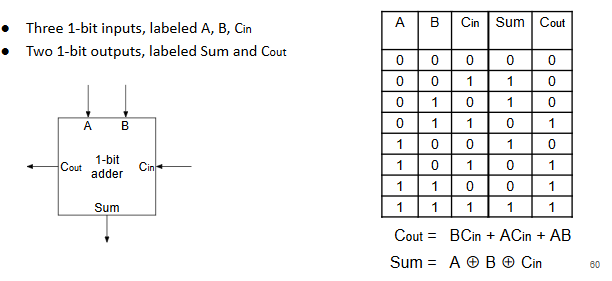
\includegraphics[width=0.5\linewidth]{一位加法器.png}
    \caption{一位加法器}
    \label{fig:enter-label}
\end{figure}
\begin{figure}
    \centering
    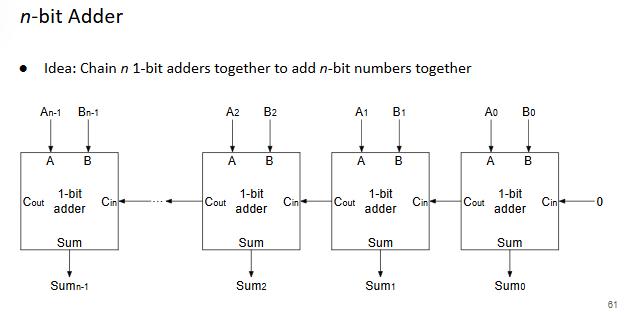
\includegraphics[width=0.5\linewidth]{n位加法器.png}
    \caption{n位加法器}
    \label{fig:enter-label}
\end{figure}
\subsubsection{有限状态机}
有限状态机是一种描述不同组件互动导致之间状态改变的数学模型概念。
有限状态机(FSM)由以下部分组成:  
- 一组状态  
- 一个转移函数:\( f(\text{当前状态}, \text{输入}) \rightarrow \text{下一状态}, \text{输出} \)  

运行有限状态机时,重复以下步骤:  
1. 接收一个输入  
2. 根据当前状态和输入,转移到下一状态并生成一个输出。
\begin{figure}
    \centering
    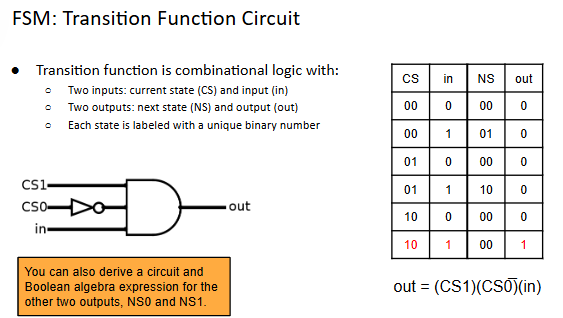
\includegraphics[width=0.5\linewidth]{图例.png}
    \caption{Enter Caption}
    \label{fig:enter-label}
\end{figure}
\begin{figure}
    \centering
    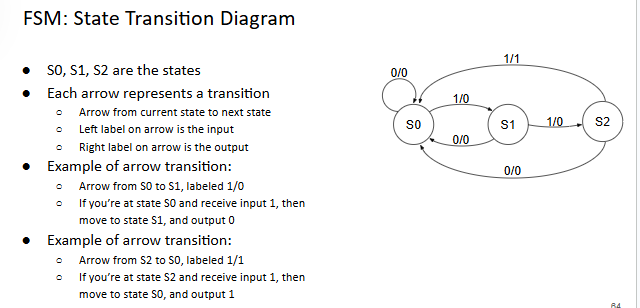
\includegraphics[width=0.5\linewidth]{有限状态机图例.png}
    \caption{有限状态机图例}
    \label{fig:enter-label}
\end{figure}
\subsubsection{从时序逻辑到同步数字系统}
注:对于逻辑组件中的信号和时间关系图来说,一位的组件图比较明确,多位的话不同位之间相互影响,可能导致很复杂\par
同步(Synchronous):彼此在时间上同步,同时发生,同步进行。
数字(Digital):对于信号而言,仅采用离散值(即非连续值)。
与采用中间值(连续值)的模拟(analogue)信号不同。
系统(Systems):由一组相互依赖的元素构成的整体。
同步数字系统(Synchronous Digital System):作为一个更大整体的一部分,其组成元素在时间上相互同步,并产生离散信号输出的系统。
时钟(Clock):在 0 和 1 之间交替的信号。
上升沿(Rising edge):时钟信号从 0 切换到 1 的时刻。
下降沿(Falling edge):时钟信号从 1 切换到 0 的时刻。
时钟周期(Clock period):相邻两个上升沿之间的时间间隔。
时钟频率(Clock frequency):每秒内上升沿出现的次数,频率 = 1 / 周期。
flipflop(触发器)作为在上升沿时刻录入此时D输入值的组件。
输入:
单比特值 D
单比特时钟信号(通常用三角形符号表示)
输出:
单比特值 Q
行为:
在时钟的上升沿时刻,将 Q 设置为 D 的值。
在其他所有时刻,输出 Q 保持不变。
用途:
**存储数据**:在两次上升沿之间,输出端 Q 的值会保持稳定。  
**控制数据流**:将输入端 D 的数据保持到下一个上升沿到来(才会更新输出)。
\begin{figure}
    \centering
    \includegraphics[width=0.5\linewidth]{触发器行为时间图.png}
    \caption{触发器行为时间图}
    \label{fig:enter-label}
\end{figure}

翻译:  
**n位寄存器(n-bit register)**:由n个触发器(flip-flop)组合而成的电路。  
- 每个触发器存储1位数据,寄存器总共存储n位数据。  

#### 输入:  
- n位输入值 **D**  
- 1位时钟信号(clock)  

#### 输出:  
- n位输出值 **Q**  

#### 行为:  
- 在时钟的上升沿(rising edge),将输出 **Q** 设置为输入 **D** 的值。  
- 在其他所有时刻,输出 **Q** 保持不变(维持上一次上升沿时采样的值)。  


### 关键概念:  
- **寄存器的本质**:通过多个D触发器并行组合,实现对多位数据的同步存储(所有位在同一个时钟边沿统一更新)。  
- **同步更新**:依赖时钟信号的边沿触发,确保数据在确定的时间点被采样,避免异步电路的竞争冒险问题,是同步数字系统(如CPU寄存器)的核心组件。

  
**寄存器/触发器无法立即将D输入传输到Q输出。**  
**时钟到输出延迟(clk-to-q delay)**:时钟上升沿到来后,Q输出完成变化所需的时间。  

### 原因讲解:  
1. **电路物理延迟的必然性**:  
   触发器(Flip-Flop)和寄存器由晶体管、逻辑门等物理器件构成,而信号在这些器件中的传播需要时间。例如:  
   - 晶体管从截止(Cutoff)到导通(Saturation)或反之,需要时间完成电荷的积累或释放(如栅极电容的充放电)。  
   - 信号每经过一个逻辑门(如与非门、反相器),都会引入**门延迟**(Gate Delay),触发器内部通常包含多级门电路(如D触发器的边沿检测电路、锁存器结构)。  

2. **触发器的内部结构决定**:  
   以D触发器为例,其典型结构包含**边沿检测电路**(如基于与非门的边沿触发器)和**锁存器**(Latch):  
   - 时钟上升沿到来时,边沿检测电路首先检测到时钟信号的变化,这一过程需要时间。  
   - 检测到边沿后,输入D的值需要通过锁存器的逻辑路径传递到输出Q,路径上的每一级门电路都会累积延迟。  

3. **信号稳定的时序要求**:  
   在同步数字系统中,触发器的输出必须在时钟边沿之后的一段时间内**稳定下来**,以确保后续电路(如下一级寄存器或组合逻辑)能正确采样数据。如果传输是“立即”的,反而会导致以下问题:  
   - 时钟边沿可能在信号尚未稳定时被下一级电路采样,引发**亚稳态**(Metastability)——输出在有效逻辑电平(0/1)之间振荡,导致系统错误。  
   - 违反电路的**建立时间**(Setup Time)和**保持时间**(Hold Time)约束,破坏时序一致性。  

4. **半导体物理的限制**:  
   即使在纳米级工艺下,信号在硅片上的传播速度也受限于光速(约0.1m/ns),例如1cm的导线传播延迟约为30ps。触发器内部的导线和晶体管尺寸虽小,但累积的延迟仍不可忽略。  


### 总结:  
clk-to-q延迟是触发器和寄存器的固有属性,由电路的物理特性(门延迟、信号传播)和同步系统的时序要求共同决定。这一延迟是设计数字系统(如CPU、存储器)时必须考虑的关键参数,直接影响时钟频率和系统稳定性——时钟周期必须足够长,以确保在下次边沿到来前,所有触发器的输出已稳定。\par
任何有时钟控制的元件都称为状态元件(需要时间相关组件才能工作)\par
示例:触发器(flip-flops)和寄存器(registers)
组合逻辑元件无需时钟即可工作(持续根据输入即时计算输出)
示例:逻辑门(logic gates)\par
组合逻辑电路具有传播延迟:输入变化后输出发生变化所需的时间。
示例:将输出 Out 设为 A + B 的加法器电路:
传播延迟的原因与实例解析:
什么是传播延迟(Propagation Delay)?
组合逻辑电路由逻辑门(如与门、或门、非门)构成,信号每经过一个门电路都会引入门延迟(Gate Delay)。传播延迟是输入信号变化后,输出信号稳定到正确值所需的总时间,等于信号从输入到输出路径上所有门延迟的累积。
考虑一个逻辑电路的逻辑延迟,应该考虑所有并行路线中最长的那个部分的延迟,

\begin{figure}
    \centering
    \includegraphics[width=0.5\linewidth]{建立时间和保存时间.png}
    \caption{建立时间和保存时间}
    \label{fig:enter-label}
\end{figure}
建立时间(Setup Time)\par
定义:建立时间指的是在时钟信号的有效边沿(如上升沿或下降沿)到来之前,输入信号(例如 D 触发器中的 D 输入)必须保持稳定不变的最小时间。只有当输入信号在这个时间内保持稳定,触发器才能正确地将输入信号采样并存储到输出端。
作用:确保在时钟信号触发时,输入信号已经稳定下来,这样触发器才能准确地读取输入值。如果输入信号在时钟有效边沿到来之前没有满足建立时间的要求,可能会导致触发器进入亚稳态(Metastability),即输出既不是逻辑高电平也不是逻辑低电平,而是处于一个不稳定的中间状态,这可能会引发后续电路的错误操作。
示例:假设有一个 D 触发器,其建立时间为 2ns。当时钟信号的上升沿即将到来时,D 输入信号必须在上升沿之前至少 2ns 就保持稳定,否则触发器可能无法正确采样该输入信号。\par
保持时间(Hold Time)\par
定义:保持时间是指在时钟信号的有效边沿到来之后,输入信号必须继续保持稳定不变的最小时间。这是为了确保触发器在完成采样操作后,输入信号不会立即发生变化,从而影响到已经存储在触发器中的值。
作用:防止在时钟信号触发后,输入信号的突然变化干扰到触发器对输入信号的正确存储。如果输入信号在时钟有效边沿之后没有满足保持时间的要求,同样可能会导致触发器输出不稳定或出现错误。
示例:若一个 D 触发器的保持时间为 1ns,那么在时钟信号的上升沿到来之后,D 输入信号需要至少保持 1ns 的稳定,以保证触发器能够正确地存储该输入值。\par




### 最大化时钟频率  \par
- 建立时间和组合延迟约束:  
时钟周期 ≥ 时钟到Q输出的延迟 + 最长组合延迟 + 建立时间  
    - 在上升沿之后,我们必须等待时钟到Q输出的延迟,以便Q输出发生变化。  
    - 然后,我们必须等待最长组合延迟,以便结果出现在D输入。  
    - 接着,我们必须让D输入在建立时间内保持稳定。  

### 满足保持时间约束 \par
- 保持时间约束:  
保持时间 ≤ 时钟到Q输出的延迟 + 最短组合延迟  
    - 在上升沿之后,我们必须等待时钟到Q输出的延迟,以便Q输出发生变化。  
    - 然后,在最短组合延迟之后,D输入之一将改变。  
    - 我们需要在D输入改变时,保持时间已经结束。 
    \begin{figure}
        \centering
        \includegraphics[width=0.5\linewidth]{选择器电路.png}
        \caption{选择器电路}
        \label{fig:enter-label}
    \end{figure}
    \subsubsection{ALU逻辑运算单元}
    \begin{figure}
        \centering
        \includegraphics[width=0.5\linewidth]{ALU简图.png}
        \caption{Enter Caption}
        \label{fig:enter-label}
    \end{figure}
    



### 算术逻辑单元(ALU)设计:拆分位  
我们可以将较长的输入拆分成较小的位组来进行操作。  
**示例**:A和B是3位输入。我们将它们拆分为单个位以执行3位按位与(AND)操作,然后重新组合结果以生成输出。 \par
\begin{figure}
    \centering
    \includegraphics[width=0.5\linewidth]{四选择器.png}
    \caption{四选择器}
    \label{fig:enter-label}
\end{figure}
\begin{figure}
    \centering
    \includegraphics[width=0.5\linewidth]{ALU电路.png}
    \caption{ALU电路}
    \label{fig:enter-label}
\end{figure}
\end{document}